\section{Generalizing the \lstinline|put| and \lstinline|get| operations}\label{s:lvars-generalizing}

The determinism result for $\lambdaLVar$ shows that adding a store of
LVars to a deterministic language substrate preserves determinism.
But, even though LVars are more general than IVars, it is not the case
that the LVar @put@/@get@ interface I've described is \emph{the most
  general} interface that preserves determinism.  In this section, I
consider some alternative semantics for @put@ and @get@ that
generalize their behavior while retaining the determinism of the
original semantics.

\subsection{Generalizing from least-upper-bound writes to inflationary, commutative writes} 

\lk{This will be about generalized inflationary+commutative writes,
  rather than least-upper-bound writes (lub is a special case of
  this).}

\TODO{Say something about how the lattice in
  Figure~\ref{f:lvars-example-lattices}(c) has different semantics if
  we have least-upper-bound writes or incremental writes, and how
  incremental writes may in fact be what is desired.  Possibly cite
  the CRDTs work and forward-reference Chapter~\ref{ch:distributed}.}

\lk{Here I can probably reuse some material from the PLDI and DISC
  papers and from my thesis proposal.}

\subsection{A more general formulation of threshold sets}\label{subsection:lvars-a-more-general-formulation-of-threshold-sets}

Certain deterministic computations are difficult to express using our
existing definition of threshold sets.  For instance, consider an LVar
that stores the result of a parallel logical ``and'' operation on two
Boolean inputs.  I'll call this data structure an \emph{\il{AndLV}},
and its two inputs the \emph{left} and \emph{right} inputs,
respectively.

We can represent the states an \il{AndLV} can take on as pairs
\il{(x,y)}, where each of \il{x} and \il{y} are \il{T}, \il{F}, or
\il{Bot}.  The \il{(Bot,Bot)} state is the state in which no input has
yet been received, and so it is the least element in the lattice of
states that our \il{AndLV} can take on, shown in
Figure~\ref{f:lvars-parallel-and}.  An additional state, \il{Top}, is
the greatest element of the lattice; it represents the situation in
which an error has occurred---if, for instance, one of the inputs
writes \il{T} and then later changes its mind to \il{F}.

\begin{figure}
\begin{center}
  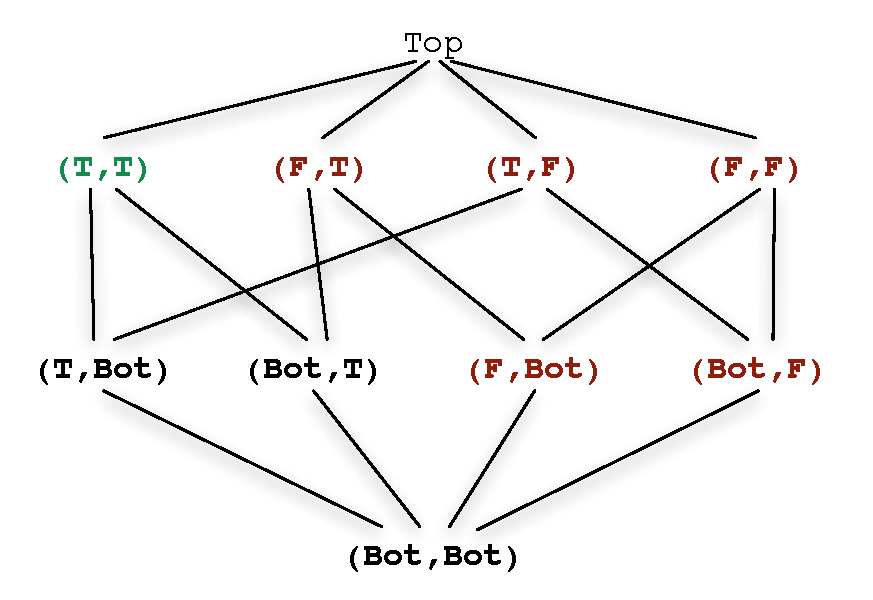
\includegraphics[width=3in]{chapter2/figures/lvars-parallel-and.pdf}
\end{center}
  \caption{Lattice of states that an \il{AndLV} can take on.  The five
    red states in the lattice correspond to a false result, and the
    one green state corresponds to a true one.}
  \label{f:lvars-parallel-and}
\end{figure}

The lattice induces a lub operation on pairs of states; for instance,
the lub of \il{(T,Bot)} and \il{(Bot,F)} is \il{(T,F)}, and the lub of
\il{(T,Bot)} and \il{(F,Bot)} is \il{Top} since the overlapping \il{T}
and \il{F} values conflict.  As usual for LVars, the @put@ operation
updates the \il{AndLV}'s state to the lub of the incoming state and
the current state.

We are interested in learning whether the result of our parallel
``and'' computation is ``true'' or ``false''.  Let's consider what
observations it is possible to make of an \il{AndLV} under our
existing definition of threshold reads.  The states \il{(T,T)},
\il{(T,F)}, \il{(F,T)}, and \il{(F,F)} are all pairwise incompatible
with one another, and so $\setof{\textrm{ \il{(T,T)}, \il{(T,F)},
    \il{(F,T)}, \il{(F,F)} }}$---that is, the set of states in which
both the left and right inputs have arrived---is a legal threshold set
argument to @get@.  The trouble with this threshold read is that it
does not allow us to get \emph{early answers} from the computation.
It would be preferable to have a @get@ operation that would ``short
circuit'' and unblock immediately if a single input of, say,
\il{(F,Bot)} or \il{(Bot,F)} was written, since no later write could
change the fact that the result of the whole computation would be
``false''.\footnote{Actually, this is not quite true: a write of
  \il{(F,Bot)} followed by a write of \il{(T,Bot)} would lead to a
  result of \il{Top}, and to the program stepping to the $\error$
  state, which is certainly different from a result of ``false''.
  But, even if a write of \il{(T,Bot)} is due to come along sooner or
  later to take the state of the \il{AndLV} to \il{Top} and thus raise
  $\error$, it should still be fine for the \il{get} operation to
  allow ``short-circuit'' unblocking, because the result of the
  \il{get} operation does not count as observable under our definition
  of observable determinism (as discussed in
  Section~\ref{subsection:lvars-errors-and-observable-determinism}).}
Unfortunately, we cannot include \il{(F,Bot)} or \il{(Bot,F)} in our
threshold set, because the resulting threshold set would no longer be
pairwise incompatible, and therefore would compromise determinism.

In order to get short-circuiting behavior from an \il{AndLV} without
compromising determinism, we need to make a slight generalization to
how threshold sets and threshold reads work.  In the new formulation,
we divide up threshold sets into subsets that we call \emph{activation
  sets}, each consisting of \emph{activation states}.  In the case of
the observation we want to make of our \il{AndLV}, one of those
activation sets is the set of states that the data structure might be
in when a state containing at least one \il{F} value has been
written---that is, the set $\setof{ \textrm{\il{(F,Bot)},
    \il{(Bot,F)}, \il{(F,T)}, \il{(T,F)}, \il{(F,F)}} }$.  When we
reach a point in the lattice that is at or above any of those states,
we know that the result will be ``false''.  The other activation set
is the singleton set $\{ \textrm{\il{(T,T)}} \}$, since we have to
wait until we reach the state \il{(T,T)} to know that the result is
``true''; a state like \il{(T,Bot)} does not appear in any of our
activation sets.

We can now redefine ``threshold set'' to mean \emph{a set of
  activation sets}.  Under this definition, the entire threshold set
that we would use to observe the contenst of our \il{AndLV} is:
\[
\{ 
\{ \textrm{\il{(F,Bot)}, \il{(Bot,F)}, \il{(F,T)}, \il{(T,F)}, \il{(F,F)}} \},
\{ \textrm{\il{(T,T)}} \}
\}
\]
We redefine the semantics of @get@ as follows: if an LVar's state
reaches (or surpasses) any state or states in a particular activation
set in the threshold set, @get@ returns \emph{that entire activation
  set}, regardless of which of its activation states was reached. If
no state in any activation set in the threshold set has yet been
reached, the @get@ operation will block.  In the case of our
\il{AndLV}, as soon as either input writes a state containing an
\il{F}, our @get@ will unblock and return the first activation set,
that is, $\{ \textrm{\il{(F,Bot)}, \il{(Bot,F)}, \il{(F,T)},
  \il{(T,F)}, \il{(F,F)}} \}$.  Hence \il{AndLV} has the expected
``short-circuit'' behavior and does not have to wait for a second
input if the first input contains an \il{F}.  If, on the other hand,
the inputs are \il{(T,Bot)} and \il{(Bot,T)}, the @get@ will unblock
and return $\{ \textrm{\il{(T,T)}} \}$.

In a real implementation, of course, the value returned from the @get@
could be more meaningful to the client---for instance, a Haskell
implementation could return \il{False} instead of returning the actual
activation set that corresponds to ``false''.  However, the
translation from $\{ \textrm{\il{(F,Bot)}, \il{(Bot,F)}, \il{(F,T)},
  \il{(T,F)}, \il{(F,F)}} \}$ to \il{False} could just as easily take
place on the client side.  In either case, the activation set returned
from the threshold read is the same regardless of \emph{which} of its
activation states caused the read to unblock, and it is impossible for
the client to tell whether the actual state of the lattice is, say,
\il{(T,F)}, \il{(F,F)}, or some other state containing \il{F}.

As part of this new formulation based on activation sets, we need to
adjust our criterion for pairwise incompatibility of threshold sets.
Recall that the purpose of the pairwise incompatibility requirement
(see Section~\ref{subsection:lvars-communication-primitives}) was to
ensure that a threshold read would return a unique result.  We need to
generalize this requirement, since although more than one element
\emph{in the same activation set} might be reached or surpassed by a
given write to an LVar, it is still the case that writes should only
unblock a \emph{unique} activation set in the threshold set.  The
pairwise incompatibility requirement then becomes that elements in an
activation set must be \emph{pairwise incompatible} with elements in
every other activation set.  That is, for all distinct activation sets
$Q$ and $R$ in a given threshold set:
%
\[ \forall q \in Q.~\forall r \in R.~q \sqcup r = \top \]
%
In our \il{AndLV} example, there are two distinct activation sets, so
if we let $Q = \{ \textrm{\il{(T,T)}} \}$ and $R = \{
\textrm{\il{(F,Bot)}, \il{(Bot,F)}, \il{(F,T)}, \il{(T,F)},
  \il{(F,F)}} \}$, the least upper bound of \il{(T,T)} and $r$ must be
\il{Top}, where $r$ is any element of $R$.  We can easily verify that
this is the case.  Furthermore, since the lattice of states that an
\il{AndLV} can take on is finite, the join function can be verified to
compute a least upper bound.

To illustrate why we need pairwise incompatibility to be defined this
way, consider the following (illegal) ``threshold set'' that does not
meet the pairwise incompatibility criterion:
\[
\{ 
\{ \textrm{\il{(F,Bot)}, \il{(Bot,F)}} \},
\{ \textrm{\il{(T,Bot)}, \il{(Bot,T)}} \}
\}
\]
A threshold read corresponding to this so-called threshold set will
unblock and return $\{ \textrm{\il{(F,Bot)}, \il{(Bot,F)}} \}$ as soon
as a state containing an \il{F} is reached, and $\{
\textrm{\il{(T,Bot)}, \il{(Bot,T)}} \}$ as soon as a state containing
a \il{T} is reached.  If, for instance, the left input writes \il{(F,
  Bot)} and the right input writes \il{(Bot, T)}, and these writes
occur in arbitrary order, the threshold read will return a
nondeterministic result, depending on the order of the two writes.
But, with the properly pairwise-incompatible threshold set above, the
threshold read will block until the write of \il{(F, Bot)} arrives,
and then will deterministically return the ``false'' activation set,
regardless of whether the write of \il{(Bot, T)} has arrived yet.
Hence ``short-circuit'' evaluation is possible.

\lk{It'd be nice to have better terminology for these than just
  ``old-style threshold sets'' and ``new-style threshold sets''.}

Finally, we can mechanically translate old-style threshold sets into
new-style threshold sets and retain the old semantics.  In the
translation, every member of the old-style threshold set simply
becomes a singleton activation set. So, if we wanted a
non-short-circuiting threshold read under the new system, our
threshold set would simply be
\[
\{ 
\{ \textrm{\il{(T,T)}} \},
\{ \textrm{\il{(T,F)}} \},
\{ \textrm{\il{(F,T)}} \},
\{ \textrm{\il{(F,F)}} \}
\},
\]
which is legal under the new formulation.

\subsection{Generalizing from threshold sets to threshold functions}

\TODO{Write this subsection!}

\lk{This will be about "threshold functions", rather than either
  simple threshold sets or generalized threshold sets (i.e., partial
  functions that take a lattice element and are undefined for all
  inputs that are not at or above a given point in the lattice, and
  constant for all inputs that are at or above that point; both kinds
  of threshold sets are a special case of this, afaict).}
